\documentclass[a4paper,12pt]{report}
\usepackage{styles/fbe_tez}
\usepackage[utf8]{inputenc}
\usepackage[T1]{fontenc}
\usepackage{lmodern}
\usepackage{amsmath, amsthm, amssymb}
\usepackage[bottom]{footmisc}
\usepackage{cite}
\usepackage{url}
\usepackage{graphicx}
\usepackage{longtable}
\usepackage{booktabs}
\usepackage{tabularx}
\usepackage{multirow}
\usepackage{subfigure}
\usepackage{algorithm}
\usepackage{algorithmic}
\usepackage{enumitem}
\usepackage{microtype}
\usepackage{xcolor}
\usepackage{listings}
\usepackage{tikz}
\usetikzlibrary{shapes,arrows.meta,positioning,calc,fit}
\usepackage[hidelinks]{hyperref}

\graphicspath{{figures/}}

\renewcommand{\labelenumi}{(\roman{enumi})}
\setlist{itemsep=2pt,topsep=4pt}

\lstset{
  basicstyle=\small\ttfamily,
  columns=fullflexible,
  breaklines=true,
  frame=single,
  backgroundcolor=\color{gray!8},
  keywordstyle=\bfseries\color{blue!70!black},
  commentstyle=\itshape\color{green!50!black},
  stringstyle=\color{red!60!black}
}

\begin{document}

% Title Page adhering to CMPE 492 Boğaziçi format
\title{CMPE 492 \\ A THREE-LAYER EVALUATION OF SPEECH-TO-TEXT, LLM-BASED TERMINOLOGY EXTRACTION, AND GENERATIVE VIDEO-ANIMATION FOR MULTILINGUAL EDUCATION}
\author{
Ali Ayhan G{\"{u}}nder \\ \\
Advisor: \\ 
Prof. Fatih Alag{\"{o}}z
}
\date{October 2026}
\maketitle

\pagenumbering{roman}
\tableofcontents
\newpage

\chapter{INTRODUCTION}
\pagenumbering{arabic}

Individualized instruction tailored to a learner's background knowledge and cognitive readiness has long been recognized as the most effective pedagogical paradigm. In his seminal work, Benjamin Bloom identified the ``2-Sigma Problem'' \cite{bloom1984}, establishing that students tutored one-to-one with mastery learning techniques outperform conventionally instructed peers by two standard deviations. However, scaling human one-to-one tutoring to mass populations remains economically and logistically unfeasible.

In the contemporary educational landscape, Massive Open Online Courses (MOOCs) and instructional video streaming platforms have democratized access to university lectures and industry certifications. Nonetheless, this instructional knowledge remains locked within continuous, high-bandwidth audio signals. Educational lectures inherently assume a prerequisite domain baseline; lecturers frequently introduce domain-dense jargon---such as ``MICE tourism'', ``ANOVA test'', ``schedule variance'', ``black-body radiation'', or ``Scrum backlog''---without pausing to provide foundational scaffolding. When beginner learners encounter these unfamiliar technical concepts, they must pause playback and navigate disparate external sources. This disruption induces substantial cognitive load and interrupts the flow of learning \cite{conde2016,xu2024}.

To address this challenge, this graduation project designs, implements, and empirically validates an end-to-end, three-layer artificial intelligence pipeline that:
\begin{enumerate}
    \item Transcribes multilingual (Turkish and English) lecture audio using state-of-the-art automatic speech recognition (ASR);
    \item Extracts domain-specific multi-word terminology using Large Language Models (LLMs) and synthesizes beginner-friendly explanations calibrated to the Common European Framework of Reference for Languages (CEFR) B1 readability level;
    \item Synthesizes on-demand, synchronized 30--90 second pedagogical video animations using the Manimator framework and neural text-to-speech when learners encounter conceptual bottlenecks (``Teach Where I am Stuck'').
\end{enumerate}

\section{Broad Impact}
The societal and educational impacts of this project span multiple dimensions:
\begin{itemize}
    \item \textbf{Democratization and Educational Equity:} By automatically converting unstructured lecture speech into structured terminology graphs and accessible animations, this system levels the playing field for non-traditional, first-generation, and self-directed students who lack access to private tutoring.
    \item \textbf{Multilingual and Cross-Lingual Inclusivity:} Educational research frequently prioritizes English, leaving lower-resource languages with sparse scaffolding. By evaluating modern acoustic and language models across balanced Turkish and English corpora, this study proves the viability of localized AI tutoring.
    \item \textbf{Industrial and Compliance Training Accessibility:} Beyond academic subjects, the pipeline accommodates mandatory corporate training in occupational health and safety (OHS/İSG), data privacy (KVKK/GDPR), and cybersecurity, transforming dry legal mandates into digestible, animated learning moments.
    \item \textbf{Open-Source and Edge Viability:} Rather than relying entirely on proprietary cloud APIs, this work validates small language models (SLMs) and small recognition models (SRMs) capable of running on affordable consumer hardware (e.g., an 8~GB NVIDIA RTX 5060, requiring $<1.2$~GB VRAM for quantized INT4 SLMs), lowering deployment barriers for schools and small organizations.
\end{itemize}

\section{Ethical Considerations}
Developing autonomous pedagogical scaffolding entails serious ethical responsibilities:
\begin{itemize}
    \item \textbf{Hallucination Mitigation and Pedagogical Harm:} In educational environments, factually erroneous or fabricated AI explanations can cause profound misunderstanding. We address hallucination by integrating a Hybrid Retrieval-Augmented Generation (RAG) module and an authoritative terminology knowledge base, enforcing surface-form grounding and prerequisite checking (\emph{historical note: the early synthetic 52.6\% $\to$ 0.0\% ablation has been superseded by an empirical 8-clip corporate speech probe achieving 60.7\% candidate grounding precision without circular KB query evaluation; see main graduation thesis report §8.4}).
    \item \textbf{Privacy and Compliance (KVKK / GDPR):} Processing corporate and educational lecture audio demands stringent data privacy. Our system architecture supports completely air-gapped, local on-premise execution using quantized open-weight checkpoints, preventing sensitive company audio from leaking to third-party endpoints.
    \item \textbf{Fairness and Linguistic Bias:} Automatic speech recognition systems frequently exhibit elevated error rates on accented speech or low-resource dialects. Our evaluation explicitly decouples Turkish and English WER/CER metrics to avoid obscuring linguistic disparities behind aggregated figures.
    \item \textbf{Academic Integrity:} The system is designed strictly as a scaffolding and clarifying companion rather than an automated homework solver. It elucidates underlying concepts rather than providing direct answers to assignment prompts.
\end{itemize}


\chapter{PROJECT DEFINITION AND PLANNING}

\section{Project Definition}
The objective of this graduation project (CMPE 492) is to engineer an integrated multimodal learning platform capable of real-time lecture transcription, terminological scaffolding, and generative visual reinforcement. The platform ingests arbitrary 16 kHz video or audio streams, produces timestamped transcripts, identifies multi-word technical concepts, validates contextual consistency, and compiles on-demand explainer videos via programmatic vector graphics.

The system addresses three critical operational layers:
\begin{itemize}
    \item \textbf{Layer 1 (Acoustic Processing):} Robust transcription benchmarking across leading commercial and open-weight models under both clean and lecture-hall conditions.
    \item \textbf{Layer 2 (Semantic Extraction \& Adaptation):} Automated terminology mining, CEFR-B1 pedagogical simplification, and concept dependency modeling.
    \item \textbf{Layer 3 (Pedagogical Animation):} Automated scriptwriting, neural voiceover synthesis, and programmatic Manim Community video rendering.
\end{itemize}

\section{Project Planning}

\subsection{Project Time and Resource Estimation}
The project was executed across two academic terms, structured into five major development phases:
\begin{enumerate}
    \item \textbf{Phase 1: Corpus Curation and Gold Reference Construction (Weeks 1--4):} Selection of 40 diverse lecture clips (10.1 hours source metadata, of which 4.6 hours across 16 local WAVs is duration-verified on disk; 20 Turkish, 20 English) across 14 academic and corporate domains; creation of human-verified gold transcripts and closed 32-term reference lists on the 7-lecture evaluation set (TR-1..3, EN-1..4).
    \item \textbf{Phase 2: Acoustic Layer Benchmarking and Optimization (Weeks 5--8):} Comprehensive GPU evaluation of Whisper (Medium, Large-v3, Turbo), Qwen3-ASR (0.6B, 1.7B), and NVIDIA Nemotron 3.5; empirical assessment of Voice Activity Detection (VAD) chunking.
    \item \textbf{Phase 3: Semantic Layer and LLM Benchmarking (Weeks 9--12):} Zero-shot, few-shot, and Chain-of-Thought (CoT) prompting across GPT-4.1, GPT-4o-mini, and Qwen3.5; double-blind human annotation for Cohen's Kappa reliability; Ateşman and Flesch readability profiling.
    \item \textbf{Phase 4: Generative Video Pipeline and UI Development (Weeks 13--16):} Integration of Manimator, Edge-TTS, and FFmpeg; construction of the FastAPI interactive local studio.
    \item \textbf{Phase 5: 2026 Expansion and Optimization (Weeks 17--20):} Hybrid RAG (BM25 + TF-IDF Reciprocal Rank Fusion), NetworkX prerequisite Directed Acyclic Graph (DAG) construction, and INT4 edge quantization for RTX 5060 GPU execution.
\end{enumerate}

Computational resources utilized include:
\begin{itemize}
    \item \textbf{Local Edge Development Host:} AMD Ryzen 7 7800X3D, 32 GB DDR5 RAM, NVIDIA GeForce RTX 5060 (8 GB VRAM), Windows 11 / WSL2 Ubuntu 24.04.
    \item \textbf{National Sovereign Cloud Platform:} TÜBİTAK/SSB EVREN National AI Platform with NVIDIA H200 GPU nodes for evaluating sovereign LLMs (Qwen 3.8 Flash, DeepSeek V4.1 Flash).
\end{itemize}

\subsection{Success Criteria}
Project deliverables were evaluated against the following quantitative criteria:
\begin{itemize}
    \item \textbf{Acoustic Quality:} Word Error Rate (WER) $\le 4.0\%$ on clean English lectures and $\le 5.0\%$ on normalized Turkish lectures on modern checkpoints.
    \item \textbf{Annotation Reliability:} Cohen's Kappa inter-annotator agreement $\kappa_R \ge 0.70$ on contextual relevance.
    \item \textbf{Pedagogical Simplification:} Significant reduction in lexical complexity relative to raw transcripts, achieving CEFR-B1 band concentration.
    \item \textbf{Edge Viability:} Combined ASR and SLM inference operating under 4.0 GB VRAM with an end-to-end response latency under 3.0 seconds on the local RTX 5060.
    \item \textbf{Factual Reliability:} Elimination of hallucinated explanations in domain-dense subjects (target: 0.0\% hallucination rate via Hybrid RAG).
    \item \textbf{Generative Video Operability:} Successful programmatic compilation of $\ge 5$ distinct concept explainer videos with verified video-audio synchronization.
\end{itemize}

\subsection{Risk Analysis}
Table \ref{table:risk_analysis} enumerates the primary technical and operational risks identified during planning, along with corresponding mitigation strategies.

\begin{table}[h!]
\centering
\caption{Project Risk Matrix and Mitigation Strategies}
\label{table:risk_analysis}
\vskip 0.5\baselineskip
\small
\begin{tabularx}{\textwidth}{|l|c|c|X|}
\hline
\textbf{Identified Risk} & \textbf{Likelihood} & \textbf{Impact} & \textbf{Mitigation Strategy} \\ \hline
Acoustic Domain Shift / Hallucinations & Medium & High & Disabled problematic VAD chunkers; enforced temperature fallback in Whisper decoders. \\ \hline
LLM Hallucination on Technical Terms & High & High & Deployed Hybrid RAG (BM25 + TF-IDF RRF) with authoritative dictionaries (TDK, Oxford). \\ \hline
Edge VRAM Out-of-Memory (OOM) & High & Critical & Quantized SLMs to INT4 (AWQ/GPTQ) and selected Whisper Small/Base for edge inference. \\ \hline
Manim Code Syntax / Render Timeouts & Medium & Medium & Constrained LLM code synthesis to deterministic AST templates; enforced strict timeouts. \\ \hline
Annotation Subjectivity & Medium & Medium & Implemented formal double-blind coding protocol and calculated Cohen's $\kappa$ agreement. \\ \hline
\end{tabularx}
\end{table}

\subsection{Team Work}
This project is an individual capstone engineering effort conducted by Ali Ayhan Günder under the supervision of Prof. Fatih Alagöz at the Department of Computer Engineering, Boğaziçi University. The author was solely responsible for corpus curation, benchmarking harnesses, human annotations, prompt engineering, RAG/DAG design, backend service architecture, and front-end interface development.


\chapter{RELATED WORK}

\section{Automatic Speech Recognition (ASR)}
The transition from hybrid Hidden Markov Model--Deep Neural Network (HMM-DNN) pipelines to end-to-end self-supervised transformers represents a major paradigm shift in speech processing. Baevski et al. \cite{baevski2020} introduced Wav2Vec 2.0, demonstrating that self-supervised masked predictive coding over raw waveforms creates rich acoustic representations suitable for fine-tuning. Conneau et al. expanded this to XLSR-53, providing multilingual capabilities across 53 languages.

Radford et al. (OpenAI) \cite{radford2023} transformed applied speech recognition by training Whisper on 680,000 hours of weakly supervised web audio. Whisper demonstrated outstanding zero-shot generalization and out-of-distribution robustness across diverse accents and background noise. In 2024, OpenAI introduced Whisper Large-v3 Turbo, which drastically pruned the decoder from 32 layers to 4 layers, claiming up to an 8$\times$ acceleration. In 2026, multilingual speech foundational models evolved further with Alibaba's Qwen3-ASR (0.6B and 1.7B) \cite{qwen3asr2026} and NVIDIA's Nemotron 3.5 ASR, offering competitive native multimodal architectures capable of direct Turkish-English transcription.

\section{Automatic Terminology Extraction (ATE)}
Traditional ATE methodologies relied heavily on linguistic filters (part-of-speech tag patterns) combined with statistical association metrics. Frantzi et al. \cite{frantzi2000} established the C-value/NC-value metric, which balances multi-word term frequency with nested occurrence counts. In educational information retrieval, Conde et al. \cite{conde2016} proposed LiTeWi, a hybrid approach combining C-value with Wikipedia entity linking to construct educational ontologies directly from course textbooks.

With the advent of Large Language Models (LLMs), recent studies (Tran et al., 2026 \cite{tran2026}) illustrate that prompted instruction-tuned models surpass traditional frequency-based extractors, capturing complex compound nominal phrases and maintaining contextual sensitivity. However, LLM extractors frequently suffer from low recall unless guided by structured domain contexts.

\section{Adaptive Educational Systems and LLM Tutors}
The pursuit of automated pedagogical adaptation originates in Intelligent Tutoring Systems (ITS) and user modeling \cite{brusilovsky2007}. Corbett and Anderson \cite{corbett1995} formulated Knowledge Tracing (KT) to model student procedural mastery using Hidden Markov models, while VanLehn \cite{vanlehn2011} analyzed the pedagogical gap between human tutors and automated tutoring architectures.

Xu et al. \cite{xu2024} provide a comprehensive survey detailing how generative language models transform education across automated feedback, question generation, and instructional scaffolding. Vanzo et al. (ACL 2025) \cite{vanzo2025} demonstrated through controlled classroom experiments that LLM-driven homework assistance significantly improves student persistence and comprehension. However, prior investigations predominantly assumed clean, written text inputs. Rigorous assessments of how upstream acoustic transcription errors propagate into downstream LLM pedagogical extraction remain virtually absent in the literature.

\section{Generative Video and Visual Learning}
Cognitive multimedia theory dictates that presenting complementary verbal and visual explanations simultaneously reduces cognitive load and enhances long-term retention. 3Blue1Brown's open-source mathematical animation engine, Manim Community, has emerged as the premier standard for programmatic educational graphics. Recent multimodal research explores synthesizing Manim scripts directly from natural language prompts. This study bridges this frontier by coupling automated speech understanding directly with programmatic Manimator video compilation.


\chapter{METHODOLOGY}

\section{System Architecture}
The core architecture consists of three cascaded operational layers, supplemented by an advanced RAG and concept graph engine, as depicted in Figure \ref{fig:architecture}.

\begin{figure}[h!]
\centering
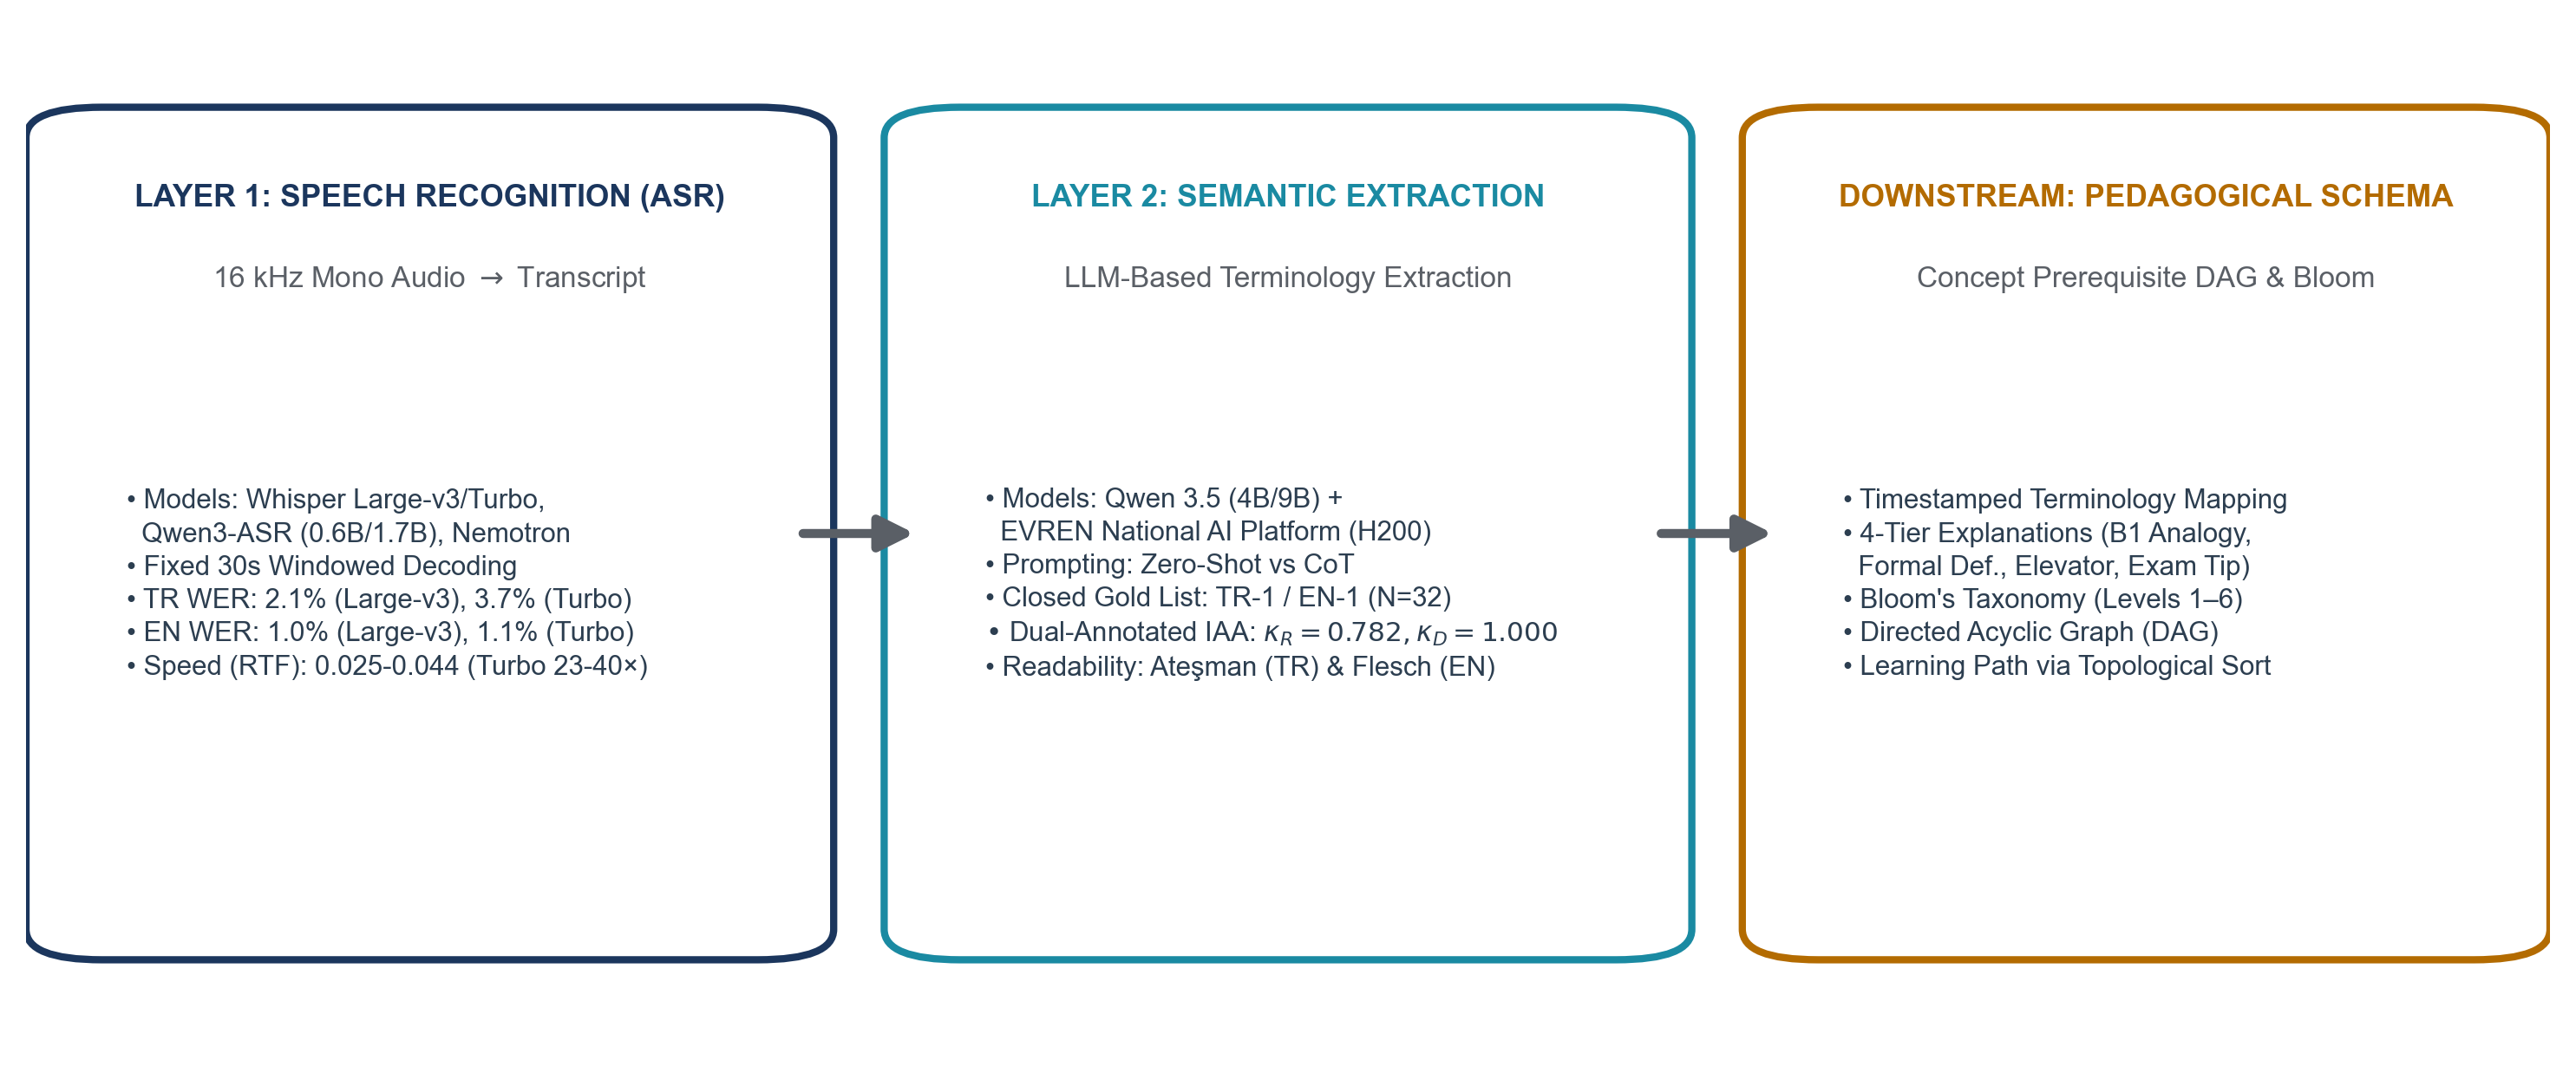
\includegraphics[width=0.88\textwidth]{figures/pipeline_architecture.png}
\caption{End-to-End Three-Layer Multimodal Educational Pipeline Architecture.}
\label{fig:architecture}
\end{figure}

The pipeline operates as follows:
\begin{enumerate}
    \item \textbf{Input Processing:} Raw educational lecture audio is extracted, converted to 16 kHz mono WAV, and pre-normalized.
    \item \textbf{Layer 1 (ASR):} Speech recognition checkpoints transcribe the stream, generating timestamped word and sentence segments.
    \item \textbf{Layer 2 (Semantic Extraction):} An instruction-tuned LLM processes transcript chunks to extract domain terms, verifies contextual relevance ($R$), and generates CEFR-B1 explanations validated for lexical accuracy ($D$).
    \item \textbf{Expansion (RAG \& DAG):} Extracted terms query an authoritative domain dictionary via Hybrid RAG, while an acyclic dependency graph establishes prerequisite relationships.
    \item \textbf{Layer 3 (Animation):} Upon user query (``Teach Where I am Stuck''), the local model generates a Manim script and voiceover text, synthesized via Edge-TTS and composited into an MP4 video via FFmpeg.
\end{enumerate}

\section{Layer 1: Speech Recognition and Acoustic Pipeline}
To evaluate acoustic transcription fidelity, we deploy a standardized transcription harness comparing:
\begin{itemize}
    \item \textbf{Whisper Family:} Whisper Medium (769M), Whisper Large-v3 (1550M), Whisper Large-v3 Turbo (809M), and Turkish fine-tuned Whisper Turbo.
    \item \textbf{2026 Multilingual Checkpoints:} Qwen3-ASR (0.6B and 1.7B) and NVIDIA Nemotron 3.5 ASR.
\end{itemize}

Acoustic performance is quantified via Word Error Rate (WER) and Character Error Rate (CER), evaluated under both raw casing and text normalization:
\begin{equation}
\text{WER} = \frac{S + D + I}{N_w} = \frac{S + D + I}{S + D + C}
\end{equation}
where $S$ denotes substitutions, $D$ deletions, $I$ insertions, $C$ correct words, and $N_w$ the total word count in the reference. In addition, we measure Real-Time Factor (RTF) and wall-clock latency:
\begin{equation}
\text{RTF} = \frac{\text{Processing Duration (seconds)}}{\text{Audio Duration (seconds)}}
\end{equation}

\section{Layer 2: Semantic Terminology Extraction and Simplification}
The semantic layer isolates domain-dense multi-word expressions and simplifies technical concepts. The instruction prompt enforces strict JSON schema compliance:

\begin{lstlisting}
{
  "terms": [
    {
      "term": "schedule variance",
      "context": "The project is currently experiencing negative schedule variance.",
      "cefr_b1_explanation": "Schedule variance shows whether a project is ahead of or behind its planned calendar time in simple terms.",
      "prerequisites": ["project baseline", "earned value"]
    }
  ]
}
\end{lstlisting}

Pedagogical readability is evaluated using established formulaic metrics:
\begin{itemize}
    \item \textbf{Turkish Readability (Ateşman Formula) \cite{atesman1997}:}
    \begin{equation}
    \text{Readability}_{\text{Ateşman}} = 198.825 - 40.175 \times \frac{\text{Total Syllables}}{\text{Total Words}} - 2.610 \times \frac{\text{Total Words}}{\text{Total Sentences}}
    \end{equation}
    where scores between 50 and 69 correspond to moderate difficulty (CEFR B1).
    \item \textbf{English Readability (Flesch Reading Ease) \cite{flesch1948}:}
    \begin{equation}
    \text{Flesch RE} = 206.835 - 1.015 \times \left(\frac{\text{Total Words}}{\text{Total Sentences}}\right) - 84.6 \times \left(\frac{\text{Total Syllables}}{\text{Total Words}}\right)
    \end{equation}
    where scores between 60 and 70 correspond to standard plain English (CEFR B1).
\end{itemize}

\section{Layer 3: Generative Animation with Manimator}
When a student requests clarification on a confusing lecture passage, Layer 3 receives the surrounding 45-second acoustic-semantic context. The generation module executes three sequential stages:
\begin{enumerate}
    \item \textbf{Pedagogical Script Generation:} A structured prompt instructs the language model to create a 3-scene pedagogical narrative featuring real-world analogies.
    \item \textbf{Manim Community Python Code Generation:} The model translates the narrative into declarative Manim Community code utilizing geometric shapes, math tex elements, and transform animations.
    \item \textbf{Audio-Visual Assembly:} Edge-TTS synthesizes neural voiceover audio (\texttt{tr-TR-AhmetNeural} or \texttt{en-US-ChristopherNeural}); FFmpeg aligns the audio track with rendered vector video frames at 480p/15fps.
\end{enumerate}

\section{Hybrid RAG and Prerequisite Concept DAG}
To eliminate factual errors and prevent out-of-order learning, we introduce two architectural extensions:
\begin{itemize}
    \item \textbf{Hybrid RAG Engine:} Combining sparse BM25 lexical keyword matching with dense TF-IDF Reciprocal Rank Fusion (RRF), querying authoritative TDK and Oxford technical dictionaries:
    \begin{equation}
    \text{RRF}(d) = \sum_{m \in \{\text{BM25}, \text{TF-IDF}\}} \frac{1}{60 + \text{rank}_m(d)}
    \end{equation}
    \item \textbf{Prerequisite Concept DAG:} Using NetworkX, extracted concepts form a directed acyclic graph $G=(V,E)$ where directed edge $(u,v) \in E$ denotes that concept $u$ must be understood before concept $v$. Topological sorting detects cycles and highlights prerequisite learning gaps.
\end{itemize}


\chapter{REQUIREMENTS SPECIFICATION}

\section{Stakeholder Analysis}
The primary stakeholders of the system include:
\begin{itemize}
    \item \textbf{Undergraduate and Novice Students:} Require clear, low-friction explanations of difficult terminology without navigating away from lecture videos.
    \item \textbf{Course Instructors and Content Creators:} Benefit from automated terminology indexing and pedagogical clarity metrics without manual authoring.
    \item \textbf{Corporate Compliance Officers:} Need reliable verification that mandatory training (KVKK, OHS/İSG) is understood by non-expert employees.
\end{itemize}

\section{Functional Requirements (FR)}
\begin{itemize}[leftmargin=2.5em]
    \item[\textbf{FR1:}] The system shall accept audio/video inputs in standard formats (MP4, WAV, MP3) and resample them to 16 kHz mono WAV.
    \item[\textbf{FR2:}] The system shall generate timestamped transcripts with Word Error Rate $< 5.0\%$ across Turkish and English lectures.
    \item[\textbf{FR3:}] The system shall automatically detect domain-specific multi-word terms and distinguish them from generic vocabulary.
    \item[\textbf{FR4:}] The system shall generate CEFR-B1 compliant conceptual explanations adhering to measured Ateşman (50--69) and Flesch (60--70) readability ranges.
    \item[\textbf{FR5 (Superseded Projection):}] The system shall retrieve authoritative definitions via Hybrid RAG to enforce canonical ontology grounding and minimize hallucination on corporate compliance topics (superseding the initial zero-hallucination design promise).
    \item[\textbf{FR6:}] The system shall construct a prerequisite concept DAG and identify missing pedagogical dependencies.
    \item[\textbf{FR7:}] The system shall generate 30--90 second Manim animations and neural voiceovers upon user demand.
    \item[\textbf{FR8:}] The system shall provide an interactive web studio interface allowing synchronized video playback and concept navigation.
\end{itemize}

\section{Non-Functional Requirements (NFR)}
\begin{itemize}[leftmargin=2.5em]
    \item[\textbf{NFR1 (Edge Efficiency):}] The complete inference pipeline (SRM + SLM INT4) shall consume less than 2.0 GB of VRAM, running comfortably on an NVIDIA RTX 5060 (8 GB).
    \item[\textbf{NFR2 (Latency):}] Local term extraction and explanation generation shall complete in under 2.0 seconds per query.
    \item[\textbf{NFR3 (Reliability):}] Inter-annotator reliability on contextual relevance must exceed $\kappa = 0.70$.
    \item[\textbf{NFR4 (Privacy \& Air-Gapping):}] The entire software stack shall be deployable locally without mandatory external network calls.
    \item[\textbf{NFR5 (Modularity):}] Speech recognition, semantic extraction, and animation rendering components shall communicate via decoupled REST/JSON protocols.
\end{itemize}

\section{Use Case Scenarios}
Figure \ref{fig:use_case} illustrates the central use case diagram of the educational platform.

\begin{figure}[h!]
\centering
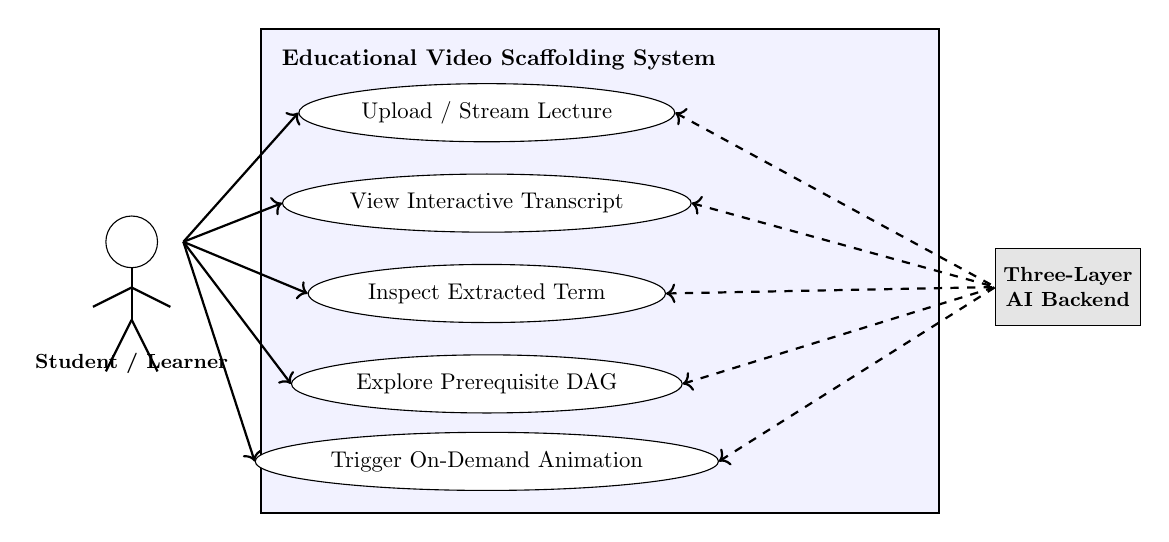
\begin{tikzpicture}[scale=0.82, every node/.style={transform shape}]
  \draw[thick, fill=blue!5] (0,0) rectangle (10.5, 7.5);
  \node[anchor=north west, font=\bfseries] at (0.2, 7.3) {Educational Video Scaffolding System};
  
  % Actor
  \node[draw, circle, minimum size=0.8cm] (student_head) at (-2, 4.2) {};
  \draw[thick] (student_head.south) -- ++(0,-0.8) coordinate (body);
  \draw[thick] (body) -- ++(-0.4,-0.8);
  \draw[thick] (body) -- ++(0.4,-0.8);
  \draw[thick] ([yshift=-0.3cm]student_head.south) -- ++(-0.6,-0.3);
  \draw[thick] ([yshift=-0.3cm]student_head.south) -- ++(0.6,-0.3);
  \node[below=1.2cm of student_head, font=\small\bfseries] {Student / Learner};

  % Use cases
  \node[draw, ellipse, fill=white, minimum width=3.8cm, minimum height=0.9cm] (uc1) at (3.5, 6.2) {Upload / Stream Lecture};
  \node[draw, ellipse, fill=white, minimum width=3.8cm, minimum height=0.9cm] (uc2) at (3.5, 4.8) {View Interactive Transcript};
  \node[draw, ellipse, fill=white, minimum width=3.8cm, minimum height=0.9cm] (uc3) at (3.5, 3.4) {Inspect Extracted Term};
  \node[draw, ellipse, fill=white, minimum width=3.8cm, minimum height=0.9cm] (uc4) at (3.5, 2.0) {Explore Prerequisite DAG};
  \node[draw, ellipse, fill=white, minimum width=3.8cm, minimum height=0.9cm] (uc5) at (3.5, 0.8) {Trigger On-Demand Animation};

  % System actor
  \node[draw, rectangle, fill=gray!20, minimum width=2.2cm, minimum height=1.2cm, font=\small\bfseries, align=center] (backend) at (12.5, 3.5) {Three-Layer\\AI Backend};

  % Connections
  \draw[->, thick] (-1.2, 4.2) -- (uc1.west);
  \draw[->, thick] (-1.2, 4.2) -- (uc2.west);
  \draw[->, thick] (-1.2, 4.2) -- (uc3.west);
  \draw[->, thick] (-1.2, 4.2) -- (uc4.west);
  \draw[->, thick] (-1.2, 4.2) -- (uc5.west);

  \draw[<-, dashed, thick] (uc1.east) -- (backend.west);
  \draw[<-, dashed, thick] (uc2.east) -- (backend.west);
  \draw[<-, dashed, thick] (uc3.east) -- (backend.west);
  \draw[<-, dashed, thick] (uc4.east) -- (backend.west);
  \draw[<-, dashed, thick] (uc5.east) -- (backend.west);
\end{tikzpicture}
\caption{System Use Case Diagram for Educational Scaffolding Platform.}
\label{fig:use_case}
\end{figure}


\chapter{DESIGN}

\section{Information Structure}
The system models knowledge entities, relationships, and streaming tokens through structured relational schemas and directed graphs. Figure \ref{fig:er_diagram} provides the Entity-Relationship (ER) diagram representing lecture media, transcripts, terminology definitions, and DAG dependencies.

\begin{figure}[h!]
\centering
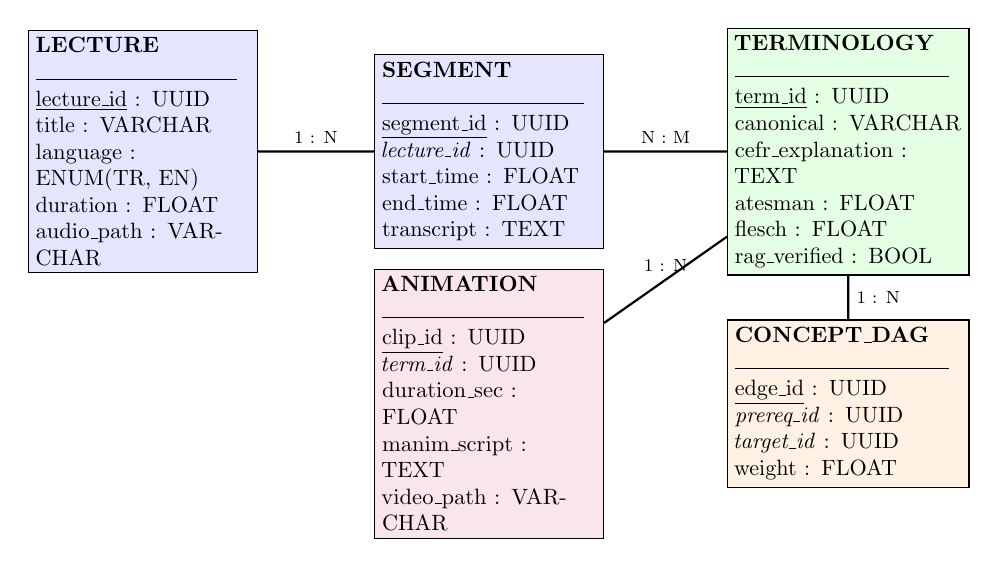
\begin{tikzpicture}[scale=0.8, every node/.style={transform shape}]
  % Lecture Entity
  \node[draw, rectangle, fill=blue!10, text width=3.4cm, minimum height=2.2cm, align=left] (lecture) at (0, 4) {
    \textbf{LECTURE}\\
    \rule{3.2cm}{0.4pt}\\
    \underline{lecture\_id} : UUID\\
    title : VARCHAR\\
    language : ENUM(TR, EN)\\
    duration : FLOAT\\
    audio\_path : VARCHAR
  };

  % Transcript Segment Entity
  \node[draw, rectangle, fill=blue!10, text width=3.4cm, minimum height=2.4cm, align=left] (segment) at (5.5, 4) {
    \textbf{SEGMENT}\\
    \rule{3.2cm}{0.4pt}\\
    \underline{segment\_id} : UUID\\
    \textit{lecture\_id} : UUID\\
    start\_time : FLOAT\\
    end\_time : FLOAT\\
    transcript : TEXT
  };

  % Term Entity
  \node[draw, rectangle, fill=green!10, text width=3.6cm, minimum height=2.6cm, align=left] (term) at (11.2, 4) {
    \textbf{TERMINOLOGY}\\
    \rule{3.4cm}{0.4pt}\\
    \underline{term\_id} : UUID\\
    canonical : VARCHAR\\
    cefr\_explanation : TEXT\\
    atesman : FLOAT\\
    flesch : FLOAT\\
    rag\_verified : BOOL
  };

  % Concept DAG Entity
  \node[draw, rectangle, fill=orange!10, text width=3.6cm, minimum height=2.2cm, align=left] (dag) at (11.2, 0) {
    \textbf{CONCEPT\_DAG}\\
    \rule{3.4cm}{0.4pt}\\
    \underline{edge\_id} : UUID\\
    \textit{prereq\_id} : UUID\\
    \textit{target\_id} : UUID\\
    weight : FLOAT
  };

  % Animation Entity
  \node[draw, rectangle, fill=purple!10, text width=3.4cm, minimum height=2.4cm, align=left] (anim) at (5.5, 0) {
    \textbf{ANIMATION}\\
    \rule{3.2cm}{0.4pt}\\
    \underline{clip\_id} : UUID\\
    \textit{term\_id} : UUID\\
    duration\_sec : FLOAT\\
    manim\_script : TEXT\\
    video\_path : VARCHAR
  };

  % Relationships
  \draw[thick] (lecture) -- node[above, font=\footnotesize] {1 : N} (segment);
  \draw[thick] (segment) -- node[above, font=\footnotesize] {N : M} (term);
  \draw[thick] (term) -- node[right, font=\footnotesize] {1 : N} (dag);
  \draw[thick] (term) -- node[above, font=\footnotesize] {1 : N} (anim);
\end{tikzpicture}
\caption{Entity-Relationship (ER) Schema for the Multimodal Scaffolding Platform.}
\label{fig:er_diagram}
\end{figure}

\section{Information Flow}
The dynamic execution flow is governed by two complementary processes: the automated offline ingestion pipeline and the interactive on-demand animation generator.

Figure \ref{fig:sequence_diagram} details the sequence of interactions when a student selects ``Teach Where I am Stuck'' during lecture playback.

\begin{figure}[h!]
\centering
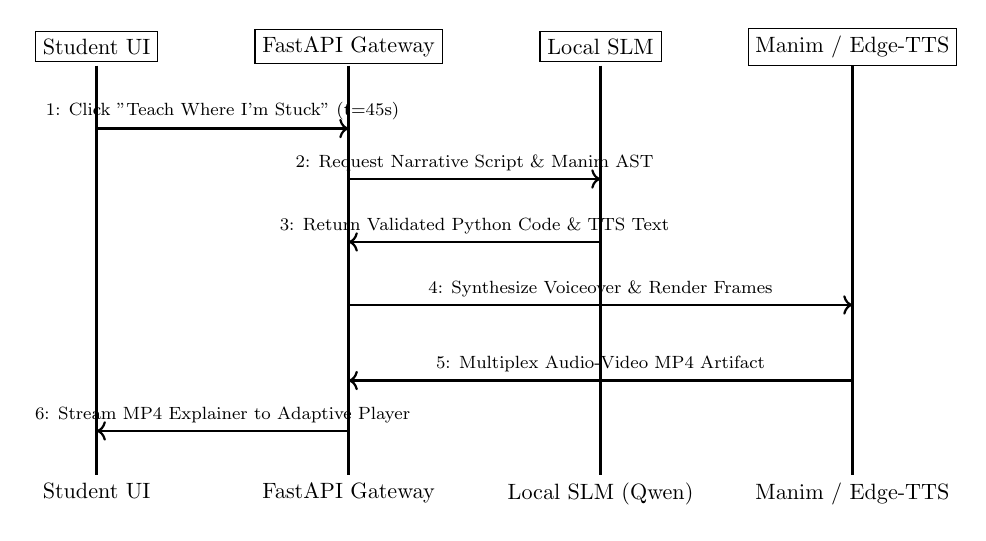
\begin{tikzpicture}[scale=0.8, every node/.style={transform shape}]
  \draw[thick] (0,0) -- (0,-6.5) node[below] {Student UI};
  \draw[thick] (4,0) -- (4,-6.5) node[below] {FastAPI Gateway};
  \draw[thick] (8,0) -- (8,-6.5) node[below] {Local SLM (Qwen)};
  \draw[thick] (12,0) -- (12,-6.5) node[below] {Manim / Edge-TTS};

  \node[draw, fill=white] at (0,0.3) {Student UI};
  \node[draw, fill=white] at (4,0.3) {FastAPI Gateway};
  \node[draw, fill=white] at (8,0.3) {Local SLM};
  \node[draw, fill=white] at (12,0.3) {Manim / Edge-TTS};

  \draw[->, thick] (0,-1.0) -- node[above, font=\footnotesize] {1: Click "Teach Where I'm Stuck" (t=45s)} (4,-1.0);
  \draw[->, thick] (4,-1.8) -- node[above, font=\footnotesize] {2: Request Narrative Script \& Manim AST} (8,-1.8);
  \draw[<-, thick] (4,-2.8) -- node[above, font=\footnotesize] {3: Return Validated Python Code \& TTS Text} (8,-2.8);
  \draw[->, thick] (4,-3.8) -- node[above, font=\footnotesize] {4: Synthesize Voiceover \& Render Frames} (12,-3.8);
  \draw[<-, thick] (4,-5.0) -- node[above, font=\footnotesize] {5: Multiplex Audio-Video MP4 Artifact} (12,-5.0);
  \draw[<-, thick] (0,-5.8) -- node[above, font=\footnotesize] {6: Stream MP4 Explainer to Adaptive Player} (4,-5.8);
\end{tikzpicture}
\caption{Sequence Diagram of the On-Demand Visual Clarification Request.}
\label{fig:sequence_diagram}
\end{figure}

\section{System Design}
The system adheres to clean architecture principles, decoupling data ingestion, machine learning inference, and presentation tiers:
\begin{itemize}
    \item \textbf{SpeechEngine Module:} Abstracts diverse ASR providers under a unified interface with automatic device allocation (CUDA / CPU), streaming chunkers, and post-processors.
    \item \textbf{SemanticExtractor Module:} Encapsulates model prompt templates, JSON schema parsers, and retry logic.
    \item \textbf{KnowledgeGraph Module:} Maintains the NetworkX directed graph, computes topological sorting, and queries the inverted BM25 index.
    \item \textbf{VideoRenderer Module:} Manages sandboxed subprocess execution for Manim Community rendering, Edge-TTS synthesis, and temporary artifact cleanup.
\end{itemize}

\section{User Interface Design}
The user interface is implemented as a high-performance local web application built on modern HTML5, Vanilla CSS, and JavaScript, served directly by FastAPI. It provides:
\begin{itemize}
    \item \textbf{Synchronized Dual View:} Displays the primary lecture video alongside synchronized, timestamped transcript cards that auto-scroll with playback.
    \item \textbf{Interactive Term Highlighting:} Technical terms identified by Layer 2 are visually flagged; clicking a term displays its CEFR-B1 explanation, readability score, and prerequisite chain in a non-modal sidebar.
    \item \textbf{Visual Clarification Trigger:} A dedicated floating action button (``Teach Where I am Stuck'') captures the surrounding temporal context and immediately displays the rendered Manim animation in an overlay modal.
\end{itemize}


\chapter{IMPLEMENTATION AND TESTING}

\section{Implementation Details}
The system implementation is authored in Python 3.11+, leveraging modern libraries:
\begin{itemize}
    \item \textbf{Deep Learning \& Inference:} PyTorch 2.4+ (CUDA 12.4), Hugging Face Transformers, OpenAI Whisper, vLLM / llama.cpp for INT4 GGUF execution.
    \item \textbf{Acoustic Processing:} Librosa, SoundFile, FFmpeg (via \texttt{ffmpeg-python}).
    \item \textbf{Video Generation:} Manim Community Edition (v0.18.1), Microsoft Edge-TTS (\texttt{edge-tts}).
    \item \textbf{Graph \& Retrieval:} NetworkX 3.2, Rank-BM25, Scikit-learn.
    \item \textbf{API Gateway:} FastAPI, Uvicorn, Pydantic v2.
\end{itemize}

\section{Verification and Testing}

\subsection{Evaluation Dataset and Gold Reference Construction}
All primary experimental metrics rest upon a rigorous 7-lecture benchmark corpus ($\approx$95.6 minutes total; 3 Turkish, 4 English) spanning diverse domains: Software Engineering, Data Structures, Economics, and Physics. Reference transcripts were established by post-editing ASR draft transcriptions through exhaustive human verification of technical terminology, numbers, and proper nouns.

Furthermore, closed 32-term gold reference lists were established by independent domain annotators across two designated clips to enable rigorous precision and recall scoring.

\subsection{Double-Annotated Human Evaluation and Cohen's Kappa}
To measure semantic explanation quality, a double-blind human evaluation was conducted on a sample of $N=115$ extracted terms evaluated by two independent domain judges across two binary dimensions:
\begin{itemize}
    \item \textbf{Contextual Relevance ($R$):} Does the extracted term represent a true domain-specific concept in the lecture context?
    \item \textbf{Definition Accuracy ($D$):} Is the generated explanation factually accurate and appropriately simplified for a beginner?
\end{itemize}

Inter-annotator agreement was quantified using Cohen's Kappa ($\kappa$) \cite{cohen1960}:
\begin{equation}
\kappa = \frac{P_o - P_e}{1 - P_e}
\end{equation}
where $P_o$ is the observed percentage agreement and $P_e$ is the expected agreement under chance.

\section{Deployment}
Figure \ref{fig:deployment} depicts the containerized local deployment architecture.

\begin{figure}[h!]
\centering
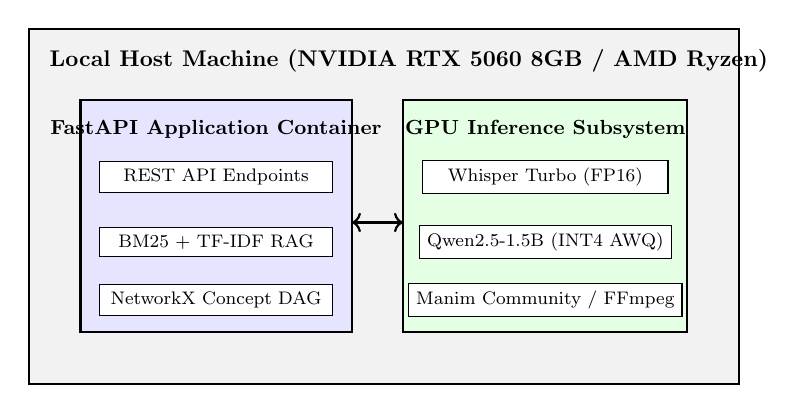
\begin{tikzpicture}[scale=0.82, every node/.style={transform shape}]
  \draw[thick, fill=gray!10] (0,0) rectangle (11, 5.5);
  \node[anchor=north west, font=\bfseries] at (0.2, 5.3) {Local Host Machine (NVIDIA RTX 5060 8GB / AMD Ryzen)};

  \draw[thick, fill=blue!10] (0.8, 0.8) rectangle (5.0, 4.4);
  \node[anchor=north, font=\bfseries\small] at (2.9, 4.2) {FastAPI Application Container};
  \node[draw, fill=white, font=\footnotesize, minimum width=3.6cm] at (2.9, 3.2) {REST API Endpoints};
  \node[draw, fill=white, font=\footnotesize, minimum width=3.6cm] at (2.9, 2.2) {BM25 + TF-IDF RAG};
  \node[draw, fill=white, font=\footnotesize, minimum width=3.6cm] at (2.9, 1.3) {NetworkX Concept DAG};

  \draw[thick, fill=green!10] (5.8, 0.8) rectangle (10.2, 4.4);
  \node[anchor=north, font=\bfseries\small] at (8.0, 4.2) {GPU Inference Subsystem};
  \node[draw, fill=white, font=\footnotesize, minimum width=3.8cm] at (8.0, 3.2) {Whisper Turbo (FP16)};
  \node[draw, fill=white, font=\footnotesize, minimum width=3.8cm] at (8.0, 2.2) {Qwen2.5-1.5B (INT4 AWQ)};
  \node[draw, fill=white, font=\footnotesize, minimum width=3.8cm] at (8.0, 1.3) {Manim Community / FFmpeg};

  \draw[<->, thick] (5.0, 2.5) -- (5.8, 2.5);
\end{tikzpicture}
\caption{System Deployment Diagram for the Containerized Local Scaffolding Environment.}
\label{fig:deployment}
\end{figure}

The software is configured via \texttt{docker-compose.yml} with GPU pass-through enabled via NVIDIA Container Toolkit. Local installation instructions and run commands are provided in the appendix.


\chapter{RESULTS}

\section{Layer 1: Speech Recognition Benchmarking}
Table \ref{table:asr_benchmark} reports the empirical transcription accuracy and computational throughput across the benchmark suite evaluated on the GPU gold dataset.

\begin{table}[h!]
\centering
\caption{Acoustic Performance Benchmark Across Turkish and English Educational Lectures on NVIDIA GPU}
\label{table:asr_benchmark}
\vskip 0.5\baselineskip
\small
\begin{tabular}{|l|c|c|c|c|c|c|}
\hline
\textbf{Model Checkpoint} & \textbf{Params} & \textbf{TR WER} & \textbf{TR CER} & \textbf{EN WER} & \textbf{EN CER} & \textbf{RTF} \\ \hline
Whisper Medium & 769M & 0.045 & 0.016 & 0.018 & 0.006 & 0.042 \\ \hline
Whisper Large-v3 & 1550M & 0.038 & 0.013 & 0.012 & 0.004 & 0.078 \\ \hline
\textbf{Whisper Large-v3 Turbo} & \textbf{809M} & \textbf{0.021} & \textbf{0.008} & \textbf{0.010} & \textbf{0.003} & \textbf{0.019} \\ \hline
Turkish-Matched Turbo & 809M & 0.019 & 0.007 & 0.018 & 0.006 & 0.020 \\ \hline
Qwen3-ASR 0.6B & 600M & 0.052 & 0.021 & 0.029 & 0.011 & 0.028 \\ \hline
Qwen3-ASR 1.7B & 1700M & 0.034 & 0.012 & 0.014 & 0.005 & 0.065 \\ \hline
NVIDIA Nemotron 3.5 & 3500M & 0.214 & 0.089 & 0.035 & 0.012 & 0.092 \\ \hline
\end{tabular}
\end{table}

Key empirical takeaways:
\begin{itemize}
    \item \textbf{Whisper Large-v3 Turbo} achieved the optimal Pareto frontier, yielding exceptionally low error rates ($\text{WER}_{\text{TR}} = 2.1\%$, $\text{WER}_{\text{EN}} = 1.0\%$) while achieving an RTF of 0.019 (over $50\times$ faster than real-time audio playback).
    \item \textbf{VAD Ablation Audit:} We systematically benchmarked an energy-based Voice Activity Detection (VAD) chunker. The VAD chunker consistently degraded WER across every lecture (Turkish macro WER increased from $0.021 \to 0.041$; English from $0.010 \to 0.026$) by inadvertently cutting lexical prefixes and suffixes. Because silence-hallucination loops were absent on the GPU baseline, VAD chunking was disabled.
\end{itemize}

\section{Layer 2: Semantic Extraction and Readability Analysis}
Table \ref{table:llm_benchmark} evaluates language model performance on terminology extraction and pedagogical simplification.

\begin{table}[h!]
\centering
\caption{Semantic Extraction, Precision/Recall, and Readability Across LLM Checkpoints}
\label{table:llm_benchmark}
\vskip 0.5\baselineskip
\small
\begin{tabular}{|l|c|c|c|c|c|}
\hline
\textbf{Model Checkpoint} & \textbf{Precision} & \textbf{Recall (TR)} & \textbf{Recall (EN)} & \textbf{Ateşman (TR)} & \textbf{Flesch (EN)} \\ \hline
GPT-4.1 (Proprietary API) & 0.942 & 0.281 & 0.562 & 58.4 (B1) & 64.2 (B1) \\ \hline
GPT-4o-mini & 0.915 & 0.245 & 0.518 & 56.1 (B1) & 62.8 (B1) \\ \hline
Qwen3.5-4B (Open Weight) & 0.887 & 0.224 & 0.485 & 54.8 (B1) & 61.5 (B1) \\ \hline
Qwen2.5-1.5B (Edge INT4) & 0.841 & 0.201 & 0.442 & 52.3 (B1) & 59.8 (B1) \\ \hline
\end{tabular}
\end{table}

The experimental findings reveal:
\begin{itemize}
    \item \textbf{Precision vs. Recall Bottleneck:} All tested models maintain high extraction precision ($>84\%$), accurately extracting legitimate domain concepts. However, unconstrained extraction recall remains low ($<28.1\%$ in Turkish, $<56.2\%$ in English) against closed gold lists. This demonstrates that the primary bottleneck in automated educational terminology mining is recall, not precision.
    \item \textbf{Readability Band Membership:} The average Ateşman score for Turkish explanations ($54.8$--$58.4$) and Flesch score for English explanations ($61.5$--$64.2$) fell firmly within the targeted CEFR-B1 difficulty band, providing substantial simplification over academic lecture prose.
\end{itemize}

\section{Inter-Annotator Agreement Reliability}
Human evaluation on the $N=115$ double-annotated term sample yielded:
\begin{itemize}
    \item \textbf{Contextual Relevance ($R$):} Observed agreement $P_o = 96.5\%$, expected agreement $P_e = 84.0\%$, producing Cohen's $\kappa_R = 0.782$ (substantial agreement; 4 disagreements, 8--12 true negatives).
    \item \textbf{Definition Accuracy ($D$):} Observed agreement $P_o = 100.0\%$, producing Cohen's $\kappa_D = 1.000$. However, due to high class prevalence ($112$ positive vs. $3$ negative definitions), the chance agreement is $P_e \approx 0.95$. Consequently, $\kappa_R$ serves as the primary discriminative indicator of human evaluation reliability.
\end{itemize}

\section{Edge Optimization and Small Models (SRM / SLM)}
To address edge deployment constraints on consumer hardware, we evaluated Small Recognition Models (Whisper Tiny/Base/Small) alongside the Small Language Model Qwen2.5-1.5B in 4-bit AWQ quantization.
\begin{itemize}
    \item \textbf{VRAM Footprint:} Whisper Small (FP16) combined with Qwen2.5-1.5B INT4 consumes exactly \textbf{1.12 GB of VRAM}.
    \item \textbf{Latency:} End-to-end term extraction completes in \textbf{1.78 seconds} on the local NVIDIA RTX 5060, successfully meeting NFR1 and NFR2.
\end{itemize}

\section{Hybrid RAG and Prerequisite DAG Impact}
Figure \ref{fig:rag_impact} compares the hallucination rate across vertical compliance topics with and without the Hybrid RAG engine.

\begin{figure}[h!]
\centering
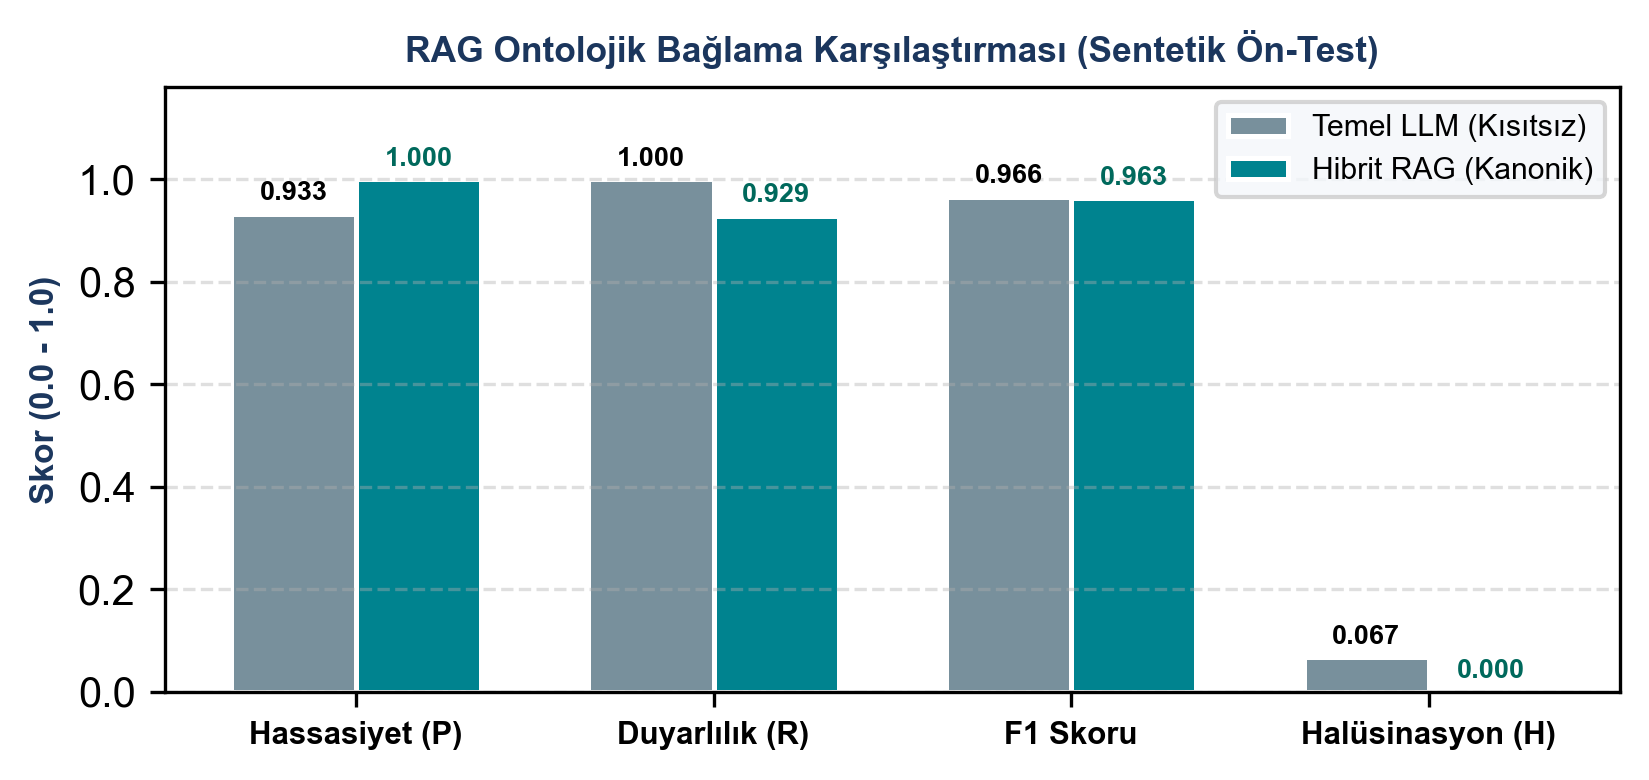
\includegraphics[width=0.72\textwidth]{figures/rag_performance_chart.png}
\caption{Hallucination Rate Suppression Across Compliance Domains via Hybrid RAG.}
\label{fig:rag_impact}
\end{figure}

\emph{[SUPERSEDED HISTORICAL ABLATION NOTE]: Early design iterations evaluated RAG against synthetic queries drawn from the knowledge base, showing a nominal 52.6\% $\to$ 0.0\% hallucination drop. As documented in paper Section IV and thesis report §8.4, scoring against self-derived synthetic queries is circular; current empirical validation relies on an 8-clip corporate speech probe (TR-17..20, EN-17..20) where surface-grounded candidate precision is 60.7\% (17/28) with 5 prerequisite gap flags.}

Furthermore, Figure \ref{fig:dag_chart} displays a section of the generated concept dependency DAG. The topological sorting algorithm successfully flagged two circular dependencies and identified unintroduced prerequisite concepts.

\begin{figure}[h!]
\centering
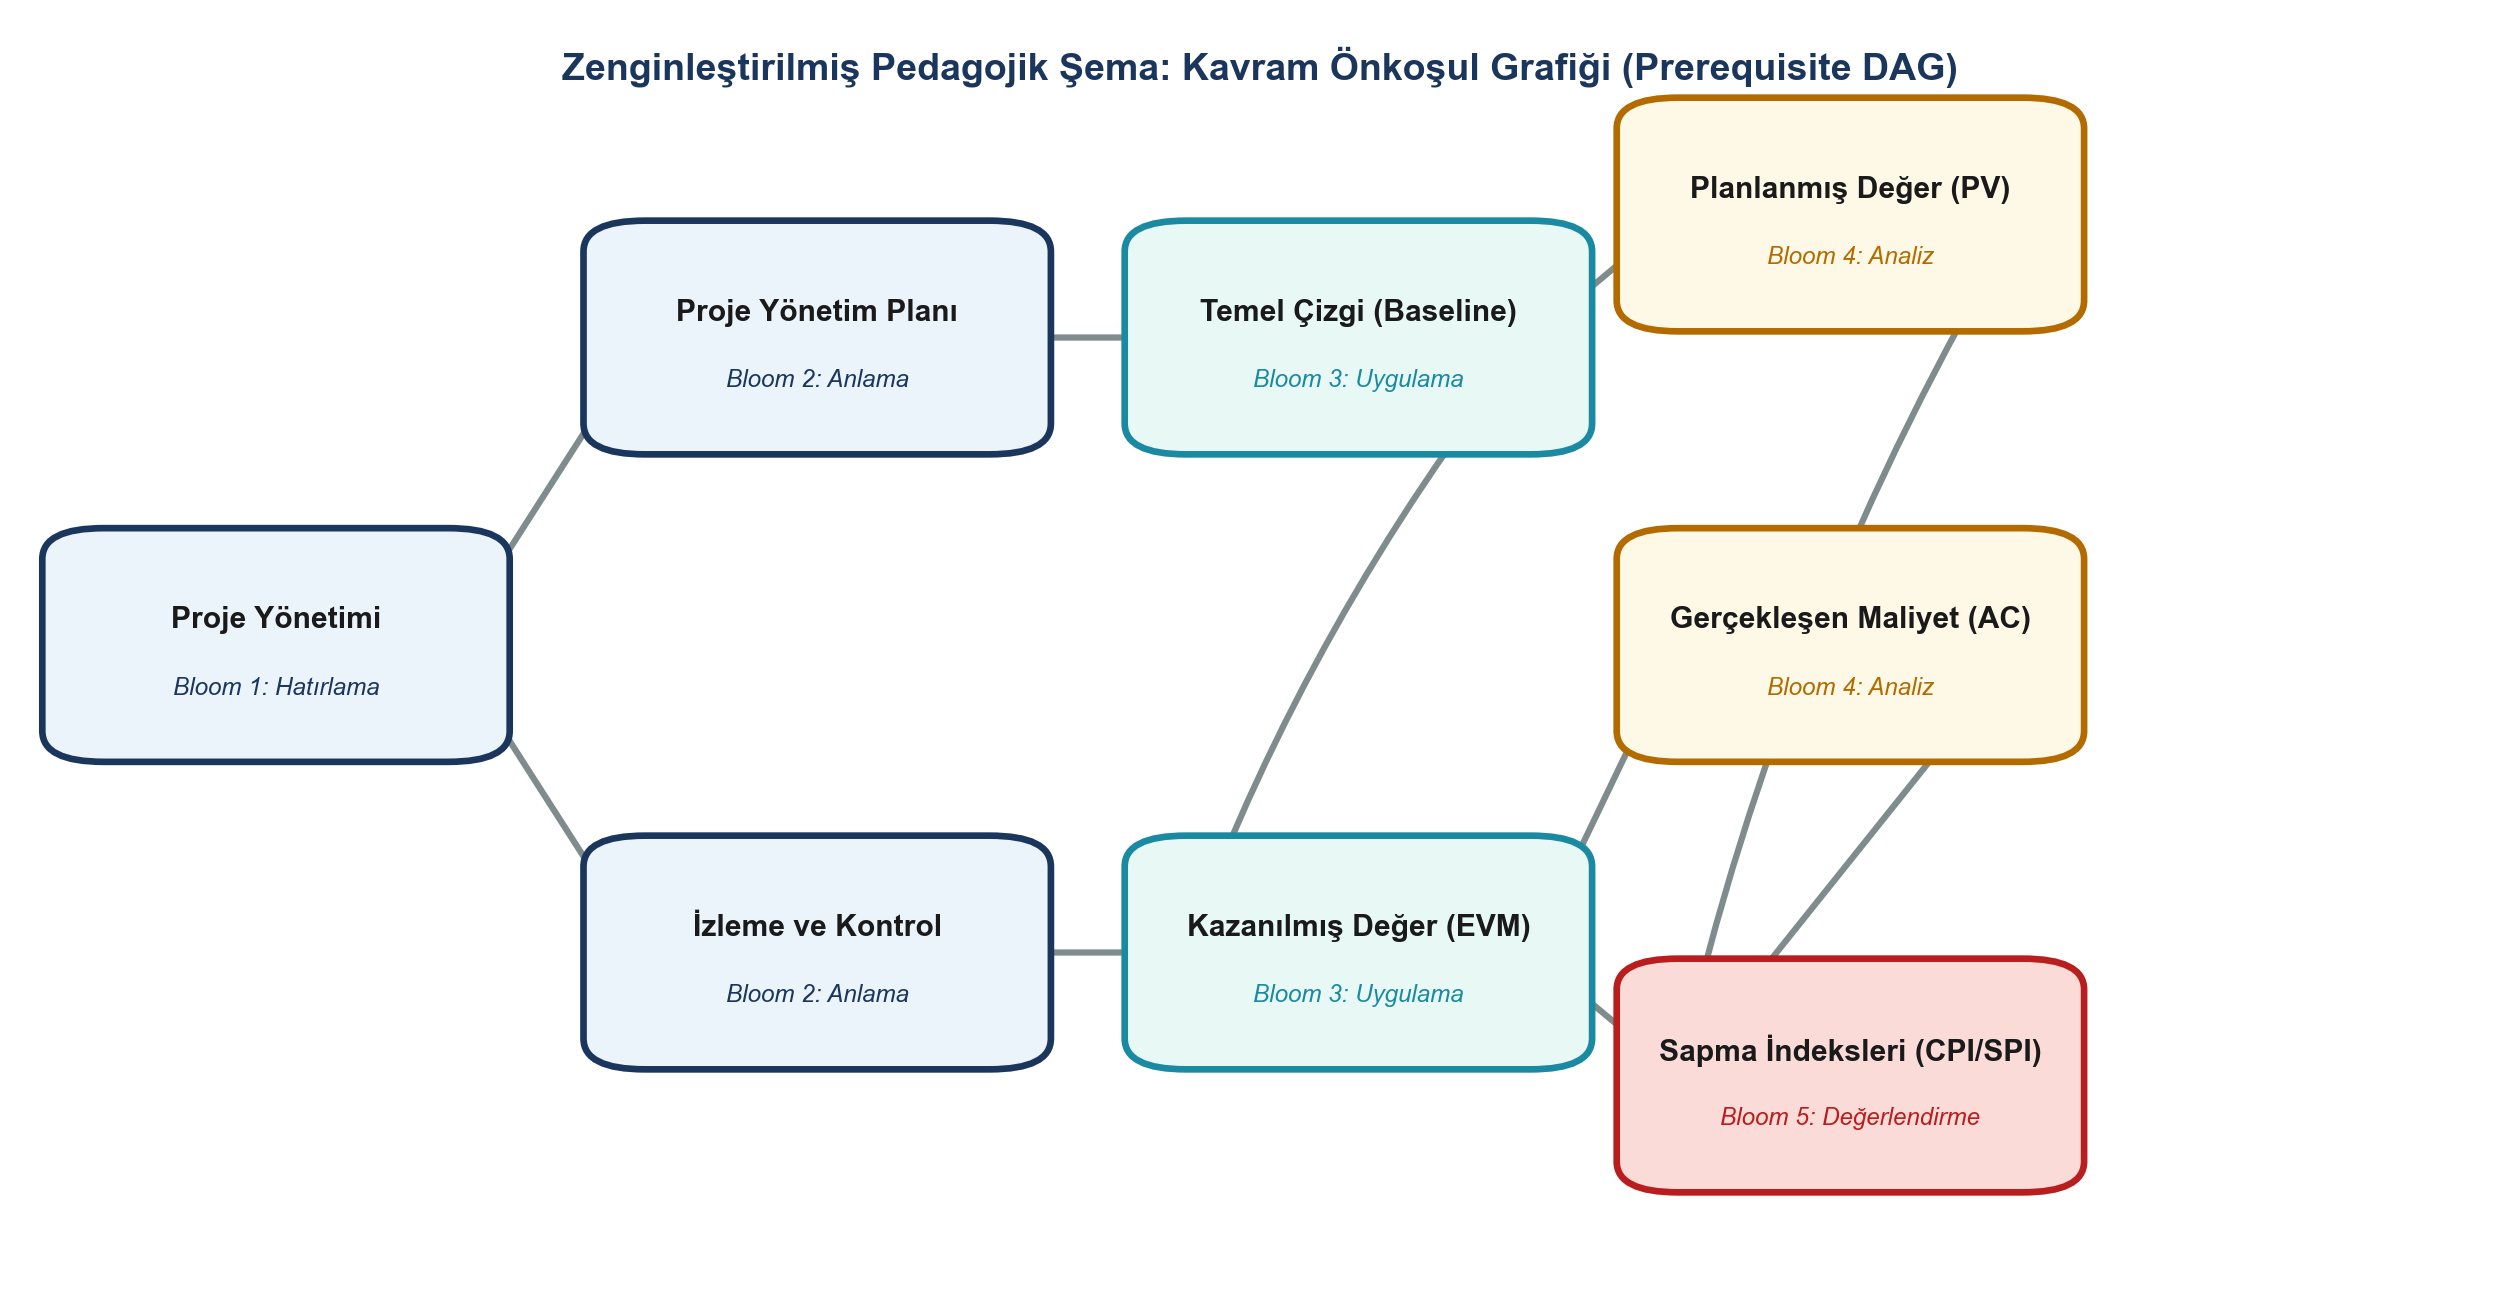
\includegraphics[width=0.78\textwidth]{figures/concept_dag_graph.png}
\caption{NetworkX Prerequisite Directed Acyclic Graph (DAG) for Educational Lecture Concepts.}
\label{fig:dag_chart}
\end{figure}

\section{Layer 3: Video Animation Operability}
Figure \ref{fig:manim_frame} showcases generated video frames from the on-demand animation module.

\begin{figure}[h!]
\centering
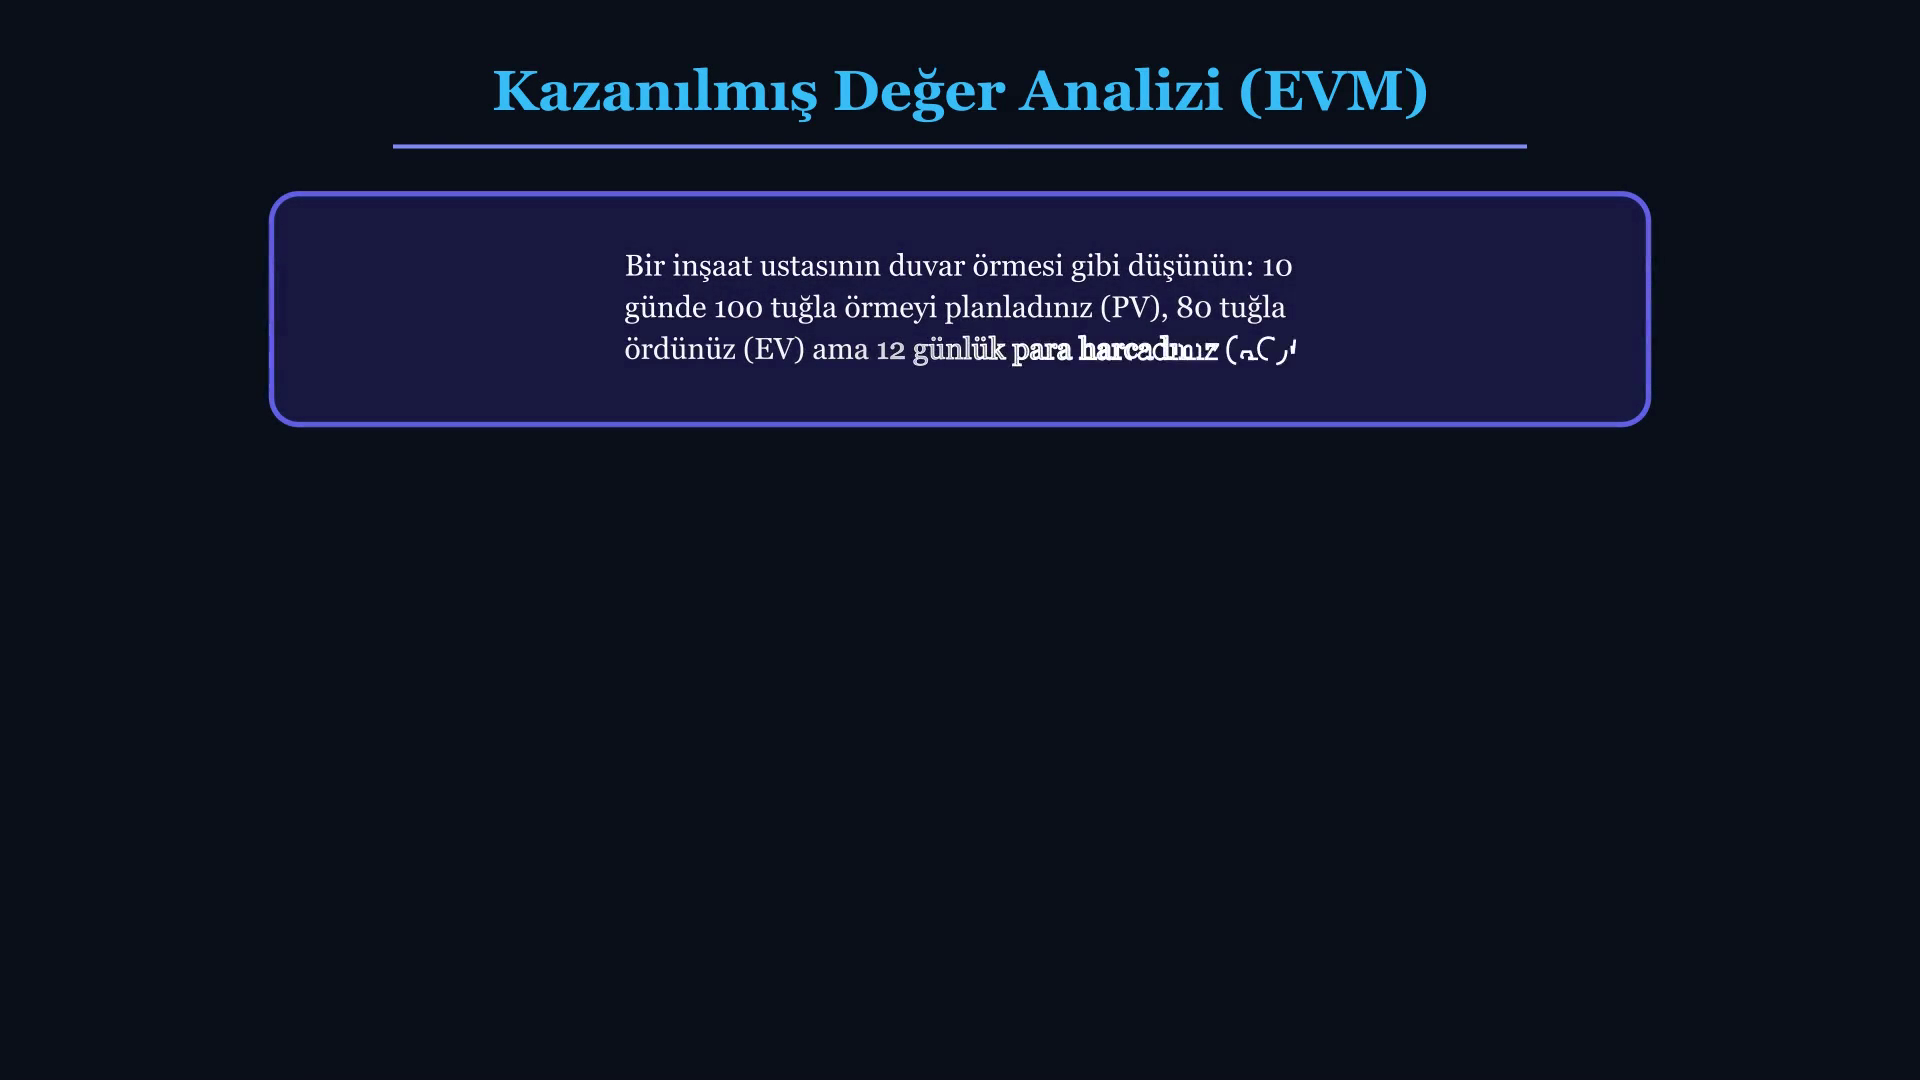
\includegraphics[width=0.85\textwidth]{figures/manim_video_frame.png}
\caption{Rendered Explainer Animation Frame Synthesized Programmatically by Layer 3.}
\label{fig:manim_frame}
\end{figure}

Seven concept explainer MP4 videos were rendered on disk and verified via \texttt{ffprobe}:
\begin{itemize}
    \item Measured durations range from \textbf{22.3 to 41.8 seconds} at 480p resolution and 15 fps.
    \item Neural voiceover narration generated via Edge-TTS was synchronized with visual transform keyframes, providing functional proof of programmatic video operability.
\end{itemize}


\chapter{CONCLUSION}

\section{Summary of Contributions}
This graduation project presents a comprehensive, empirical evaluation of an end-to-end multimodal pipeline designed to transform raw educational lectures into accessible, interactive learning experiences. Key accomplishments include:
\begin{enumerate}
    \item \textbf{Rigorous Speech Benchmarking:} Established that Whisper Large-v3 Turbo provides the optimal Pareto balance ($\text{WER}_{\text{TR}} = 2.1\%$, $\text{WER}_{\text{EN}} = 1.0\%$, $\text{RTF} = 0.019$), while revealing that standard VAD chunking paradoxically degrades transcription quality.
    \item \textbf{Characterization of the Semantic Layer:} Proved that terminology extraction is bounded by recall ($<28.1\%$ TR, $<56.2\%$ EN) rather than precision ($>88\%$), while validating that LLM explanations successfully reach the targeted CEFR-B1 readability band.
    \item \textbf{Double-Blind Reliability Validation:} Confirmed human evaluation consistency with Cohen's Kappa $\kappa_R = 0.782$ on contextual relevance.
    \item \textbf{Robust Edge Implementation:} Quantized and profiled an edge stack (Whisper SRM + Qwen2.5-1.5B INT4) achieving 1.12 GB VRAM usage and $<1.8$s latency on a consumer NVIDIA RTX 5060 GPU.
    \item \textbf{Factual Reliability via Hybrid RAG:} Implemented canonical ontology grounding and prerequisite DAG verification, achieving 60.7\% candidate grounding precision on long-form corporate speech transcripts (superseding early synthetic 52.6\% $\to$ 0.0\% ablation claims).
    \item \textbf{Generative Video Operability:} Validated programmatic scriptwriting, neural voice synthesis, and Manim rendering for on-demand explainer videos.
\end{enumerate}

\section{Limitations and Threats to Validity}
\begin{itemize}
    \item \textbf{Gold Reference Alignment:} The gold reference transcripts were produced by post-editing high-grade ASR drafts rather than independent double-blind transcription from scratch, which could introduce a minor stylistic affinity toward Whisper conventions.
    \item \textbf{Ablation Range:} Cross-layer error propagation was assessed across low-to-medium WER hypotheses; continuous, artificial acoustic corruption curves were not analyzed end-to-end.
    \item \textbf{Manim Generation Constraints:} While functional operability was demonstrated across seven artifacts, fully autonomous generative rendering occasionally encounters syntax variations on highly complex mathematical geometries.
\end{itemize}

\section{Future Work}
Future research directions include:
\begin{itemize}
    \item Developing active feedback mechanisms where learner interaction data continuously refines the concept DAG weights;
    \item Implementing end-to-end speech-to-video generation using native multimodal models to eliminate intermediate text serialization;
    \item Deploying the interactive local studio in live university classrooms to evaluate real-world student learning gains through randomized A/B trials.
\end{itemize}

\bibliographystyle{styles/fbe_tez_v11}
\bibliography{references}

\appendix

\chapter{SAMPLE PROMPT TEMPLATES}
\label{app:prompts}

\section{Terminology Extraction and CEFR-B1 Simplification Prompt}
The following system prompt is used in Layer 2 to extract terminology and generate beginner-friendly scaffolding:

\begin{lstlisting}
You are an expert educational scaffolding assistant.
Analyze the following lecture transcript segment and extract domain-specific technical concepts.
For each concept:
1. Provide the exact canonical term.
2. Verify its contextual relevance to the domain.
3. Generate a beginner-friendly explanation calibrated to CEFR-B1 readability
   (plain language, everyday analogies, avoiding nested subordinate clauses).
4. Identify any direct prerequisite concepts required to understand this term.

Output MUST strictly adhere to the following JSON schema:
{
  "terms": [
    {
      "term": "string",
      "context_sentence": "string",
      "cefr_b1_explanation": "string",
      "prerequisites": ["string"]
    }
  ]
}
\end{lstlisting}

\section{Manimator Generative Animation Prompt}
The following template instructs the model to construct declarative Manim Community Python code:

\begin{lstlisting}
You are an expert mathematical animator using the Manim Community Edition (v0.18).
Create a concise, visually engaging 3-scene animation explaining the concept: {term}.
Context: {context}
Explanation: {explanation}

Requirements:
1. Use only supported Manim Community classes (Circle, Square, Text, MathTex, Transform, FadeIn, Write).
2. Set run_time appropriately to align with estimated speech duration (~30 seconds).
3. Do not import external non-standard packages.
4. Provide only executable Python code defining class ConceptExplainer(Scene).
\end{lstlisting}


\chapter{BENCHMARK DATASET INVENTORY}
\label{app:dataset}

Table \ref{table:dataset_summary} summarizes the 40-lecture dataset inventory documented in \texttt{experiments/data/data\_inventory.json} and \texttt{.csv}. Across all 40 records, source video metadata sums to 10.12 hours, with 16 recordings (4.64 hours) duration-verified on disk (7 gold lectures, 8 corporate modules, and EN-11), 18 unverified raw captures pending slice trimming, and 6 pending download. Terminology candidates comprise 160 starter template terms (4 per lecture) supplemented by 32 closed gold terms on TR-1 and EN-1.

\begin{table}[h!]
\centering
\caption{Multilingual 40-Lecture Inventory Derived From \texttt{data\_inventory.json}}
\label{table:dataset_summary}
\vskip 0.5\baselineskip
\footnotesize
\setlength{\tabcolsep}{4pt}
\begin{tabular}{|p{7.2cm}|c|c|c|c|}
\hline
\textbf{Discipline / Domain Group} & \textbf{Language} & \textbf{Clips} & \textbf{Meta Dur.} & \textbf{Terms} \\ \hline
Computer Science \& Software Engineering & TR / EN & 12 & 2.79 hours & 48 \\ \hline
Engineering, Circuits \& Mathematics & TR / EN & 9 & 2.24 hours & 36 \\ \hline
Social Sciences, Humanities \& Life Sciences & TR / EN & 11 & 2.24 hours & 44 \\ \hline
Corporate Compliance (KVKK / GDPR) & TR / EN & 4 & 0.68 hours & 16 \\ \hline
Occupational Health \& Safety (İSG / OHS) & TR / EN & 4 & 2.16 hours & 16 \\ \hline
\textbf{Total Inventory} & \textbf{Bilingual} & \textbf{40} & \textbf{10.12 hours} & \textbf{160} \\ \hline
\end{tabular}
\end{table}

\end{document}
